\documentclass[tikz,border=6pt]{standalone}
\usepackage{tikz}
\usepackage{xcolor}
\usepackage[T1]{fontenc}
\usepackage{lmodern}
\usetikzlibrary{positioning,fit,arrows.meta,calc,backgrounds}

% ── Palette ───────────────────────────────────────────────────────────────────
\definecolor{PlannerBg}{HTML}{EBF2FA}
\definecolor{PlannerBd}{HTML}{4A86C8}
\definecolor{PlannerFg}{HTML}{1E4D8C}
\definecolor{HarnessBg}{HTML}{E8F4F1}
\definecolor{HarnessBd}{HTML}{3A9E88}
\definecolor{HarnessFg}{HTML}{1A5C4E}
\definecolor{AnalyzerBg}{HTML}{F0EBF8}
\definecolor{AnalyzerBd}{HTML}{8A63C8}
\definecolor{AnalyzerFg}{HTML}{4A1E8C}
\definecolor{ToolBg}{HTML}{FFF8E8}
\definecolor{ToolBd}{HTML}{C8963A}
\definecolor{ToolFg}{HTML}{6B4A00}
\definecolor{QCBg}{HTML}{FEF0EF}
\definecolor{QCBd}{HTML}{D95F4B}
\definecolor{QCFg}{HTML}{8C2A1E}
\definecolor{NeutralBg}{HTML}{F4F3F1}
\definecolor{NeutralBd}{HTML}{AAAAAA}
\definecolor{ArrowCol}{HTML}{555555}
\definecolor{LoopArrow}{HTML}{7B52C0}
\definecolor{IconGray}{HTML}{6E6E6E}

%% ── Master geometry ───────────────────────────────────────────────────────────
% Row centres.  A 1.38 unit pitch leaves ~0.82 units of clear space between
% consecutive 0.56-unit boxes, which is where every label and arrow route goes.
\def\yA{-1.05} \def\yB{-2.43} \def\yC{-3.81}
\def\yD{-5.19} \def\yE{-6.57}
% Harness threads share the same vertical span but sit on a tighter 0.98 pitch
\def\hyA{-1.72} \def\hyB{-2.70} \def\hyC{-3.68}
\def\hyD{-4.66} \def\hyE{-5.64}
% Frame extents.  The header band is drawn ABOVE \yTop, never over it.
\def\yTop{-0.42} \def\yBot{-7.30}
\def\pL{-1.02}  \def\pR{4.92}
\def\hL{5.42}   \def\hR{16.62}
\def\aL{17.22}  \def\aR{21.52}
\def\px{1.95}   \def\ax{19.40}

%% ── Icon macros.  Absolute placement: (x, y) is the icon's own centre, so a
%%    glyph can never be displaced by its box resizing.
\newcommand{\docicon}[2]{%
  \begin{scope}[shift={(#1,#2)}]
    \draw[line width=0.45pt, draw=IconGray, fill=white]
      (-0.055,-0.070) rectangle (0.065,0.070);
    \draw[line width=0.45pt, draw=IconGray] (0.020,0.070) -- (0.065,0.025);
    \draw[line width=0.36pt, draw=IconGray!55]
      (-0.026,0.022) -- (0.008,0.022)
      (-0.026,-0.012) -- (0.040,-0.012)
      (-0.026,-0.046) -- (0.040,-0.046);
  \end{scope}}
\newcommand{\magicon}[2]{%
  \begin{scope}[shift={(#1,#2)}]
    \draw[line width=0.55pt, draw=PlannerBd!80] (0,0.020) circle (0.060cm);
    \draw[line width=0.55pt, draw=PlannerBd!80] (0.044,-0.040) -- (0.094,-0.090);
  \end{scope}}
\newcommand{\linkicon}[2]{%
  \begin{scope}[shift={(#1,#2)}]
    \draw[line width=0.45pt, draw=ToolBd, rounded corners=0.8pt]
      (-0.046,0.016) -- (0.004,0.016) arc(90:-90:0.032) -- (-0.046,-0.048);
    \draw[line width=0.45pt, draw=ToolBd, rounded corners=0.8pt]
      (0.046,0.016) -- (-0.004,0.016) arc(90:270:0.032) -- (0.046,-0.048);
  \end{scope}}
\newcommand{\gearicon}[3]{%
  \begin{scope}[shift={(#1,#2)}]
    \draw[line width=0.42pt, draw=HarnessBd!85, fill=HarnessBg]
      (0,0) circle (0.052cm);
    \foreach \a in {#3}{%
      \draw[line width=0.36pt, draw=HarnessBd!85]
        ({0.052*cos(\a)},{0.052*sin(\a)}) -- ({0.098*cos(\a)},{0.098*sin(\a)});
    }
  \end{scope}}
\newcommand{\shieldicon}[2]{%
  \begin{scope}[shift={(#1,#2)}]
    \draw[line width=0.5pt, draw=QCBd, fill=QCBg!70]
      (0,0.092) -- (0.072,0.054) -- (0.072,-0.016)
      .. controls (0.072,-0.078) and (0.035,-0.100) .. (0,-0.100)
      .. controls (-0.035,-0.100) and (-0.072,-0.078) .. (-0.072,-0.016)
      -- (-0.072,0.054) -- cycle;
    \draw[line width=0.5pt, draw=QCFg]
      (-0.034,-0.016) -- (-0.006,0.024) -- (0.042,-0.040);
  \end{scope}}
\newcommand{\bulbicon}[2]{%
  \begin{scope}[shift={(#1,#2)}]
    \draw[line width=0.45pt, draw=AnalyzerBd, fill=AnalyzerBg!70]
      (0,0.030) circle (0.062cm);
    \draw[line width=0.45pt, draw=AnalyzerBd]
      (-0.027,0.000) -- (-0.027,-0.062) -- (0.027,-0.062) -- (0.027,0.000);
    \draw[line width=0.36pt, draw=AnalyzerBd]
      (-0.021,-0.078) -- (0.021,-0.078)
      (-0.021,-0.096) -- (0.021,-0.096);
  \end{scope}}
\newcommand{\branchicon}[2]{%
  \begin{scope}[shift={(#1,#2)}]
    \draw[line width=0.45pt, draw=AnalyzerBd] (-0.060,0.058) -- (0,-0.010);
    \draw[line width=0.45pt, draw=AnalyzerBd] (0,-0.010) -- (-0.060,-0.076);
    \draw[line width=0.45pt, draw=AnalyzerBd] (0,-0.010) -- (0.072,-0.010);
    \fill[AnalyzerBd] (0.084,-0.010) circle (0.017cm);
    \draw[line width=0.40pt, draw=AnalyzerFg]
      (-0.084,0.030) -- (-0.071,0.018) -- (-0.050,0.052);
  \end{scope}}
\newcommand{\runicon}[2]{%
  \begin{scope}[shift={(#1,#2)}]
    \draw[line width=0.45pt, draw=IconGray, fill=white, rounded corners=0.8pt]
      (-0.072,-0.054) rectangle (0.072,0.058);
    \draw[line width=0.40pt, draw=IconGray!70] (-0.072,0.034) -- (0.072,0.034);
    \fill[IconGray!70] (-0.052,0.046) circle (0.009cm);
    \fill[IconGray!70] (-0.027,0.046) circle (0.009cm);
    \fill[IconGray!85] (0,0.002) -- (0.032,-0.020) -- (0,-0.042) -- cycle;
  \end{scope}}

\begin{document}
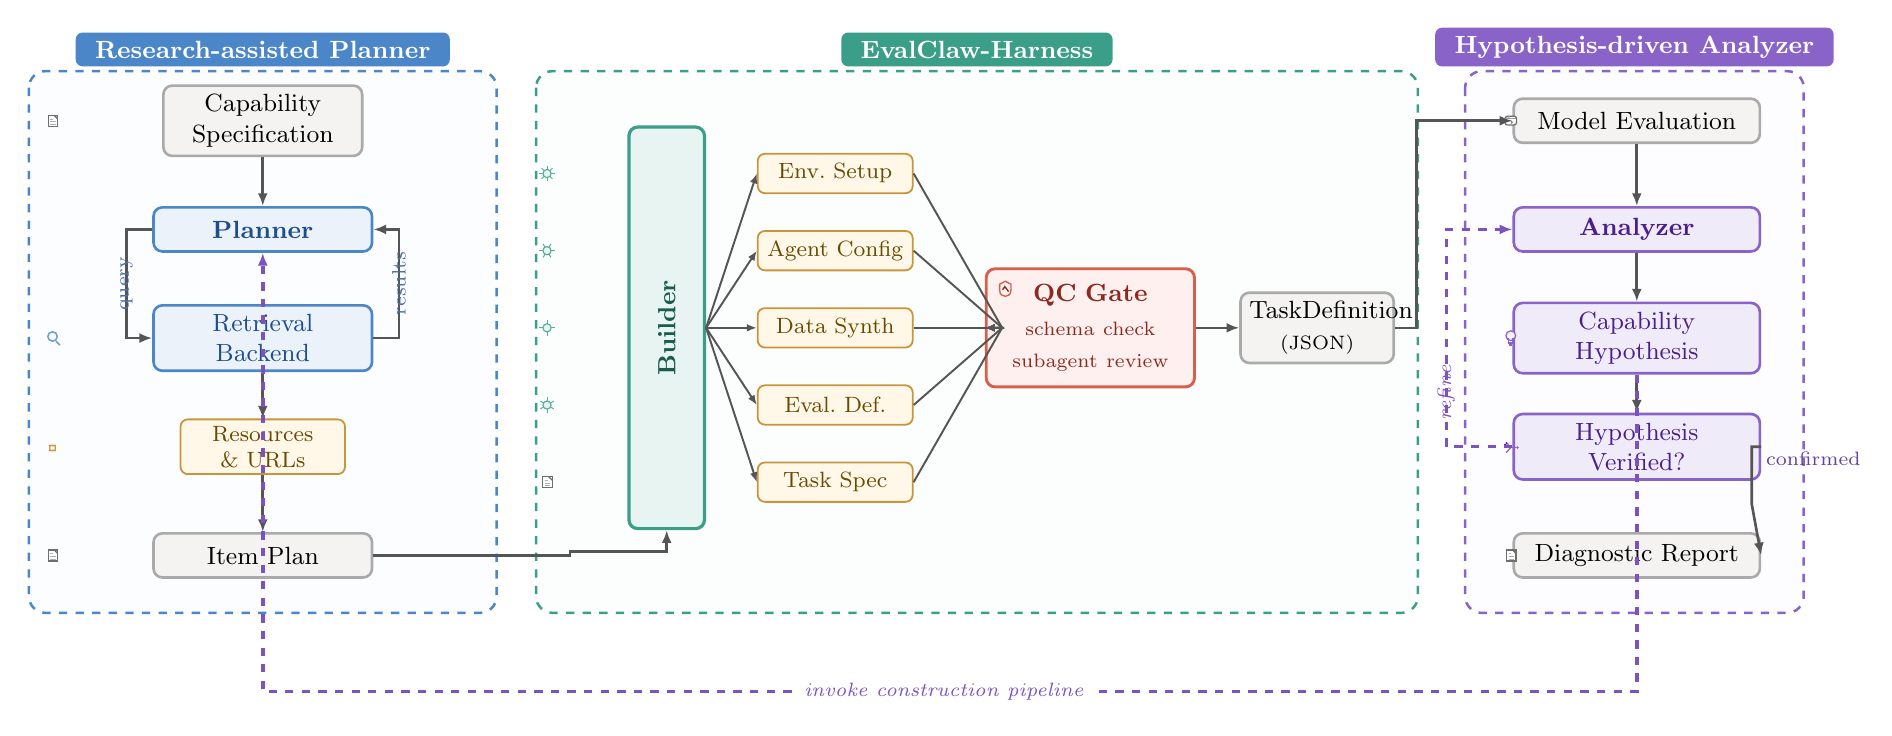
\begin{tikzpicture}[
    font=\small,
    nbox/.style   = {draw, rounded corners=3.2pt, line width=0.95pt,
                     align=center, inner sep=3.2pt, minimum height=0.56cm},
    thread/.style = {draw, rounded corners=2.6pt, line width=0.65pt,
                     align=center, inner sep=2.4pt, minimum height=0.50cm,
                     font=\footnotesize, fill=ToolBg, draw=ToolBd, text=ToolFg},
    arr/.style      = {-{Latex[length=4.6pt,width=3.6pt]}, line width=0.95pt,
                       color=ArrowCol},
    thinarr/.style  = {-{Latex[length=3.6pt,width=2.8pt]}, line width=0.7pt,
                       color=ArrowCol},
    looparr/.style  = {-{Latex[length=4.6pt,width=3.6pt]}, line width=1.0pt,
                       color=LoopArrow, dashed},
    albl/.style     = {font=\scriptsize, text=ArrowCol, inner sep=1.6pt},
    llbl/.style     = {font=\scriptsize\itshape, text=LoopArrow, inner sep=1.6pt},
  ]

%% ════════════════════════════════════════════════════════════════════════════
%%  REGION FRAMES.  The label band is anchored with `south` at \yTop, i.e. it
%%  sits entirely ABOVE the dashed frame, so it can never cover a box.
%% ════════════════════════════════════════════════════════════════════════════
\begin{scope}[on background layer]
  \draw[draw=PlannerBd, dashed, line width=0.9pt, rounded corners=6pt,
        fill=PlannerBg, fill opacity=0.13] (\pL,\yTop) rectangle (\pR,\yBot);
  \node[fill=PlannerBd, text=white, rounded corners=2.5pt, inner xsep=7pt,
        inner ysep=3pt, font=\small\bfseries, minimum width=\pR-\pL-2pt,
        anchor=south, outer sep=0pt]
    at ({(\pL+\pR)/2},\yTop+0.06) {Research-assisted Planner};

  \draw[draw=HarnessBd, dashed, line width=0.9pt, rounded corners=6pt,
        fill=HarnessBg, fill opacity=0.13] (\hL,\yTop) rectangle (\hR,\yBot);
  \node[fill=HarnessBd, text=white, rounded corners=2.5pt, inner xsep=7pt,
        inner ysep=3pt, font=\small\bfseries, minimum width=\hR-\hL-2pt,
        anchor=south, outer sep=0pt]
    at ({(\hL+\hR)/2},\yTop+0.06) {EvalClaw-Harness};

  \draw[draw=AnalyzerBd, dashed, line width=0.9pt, rounded corners=6pt,
        fill=AnalyzerBg, fill opacity=0.13] (\aL,\yTop) rectangle (\aR,\yBot);
  \node[fill=AnalyzerBd, text=white, rounded corners=2.5pt, inner xsep=7pt,
        inner ysep=3pt, font=\small\bfseries, minimum width=\aR-\aL-2pt,
        anchor=south, outer sep=0pt]
    at ({(\aL+\aR)/2},\yTop+0.06) {Hypothesis-driven Analyzer};
\end{scope}

%% ════════════════════════════════════════════════════════════════════════════
%%  COLUMN 1 — Research-assisted Planner
%% ════════════════════════════════════════════════════════════════════════════
\node[nbox, fill=NeutralBg, draw=NeutralBd, text=black, text width=2.30cm]
  (capspec) at (\px,\yA) {Capability Specification};
\node[nbox, fill=PlannerBg, draw=PlannerBd, text=PlannerFg, text width=2.55cm]
  (planner) at (\px,\yB) {\textbf{Planner}};
\node[nbox, fill=PlannerBg, draw=PlannerBd, text=PlannerFg, text width=2.55cm]
  (retrieval) at (\px,\yC) {Retrieval Backend};
\node[thread, text width=1.92cm, minimum height=0.52cm]
  (resources) at (\px,\yD) {Resources \& URLs};
\node[nbox, fill=NeutralBg, draw=NeutralBd, text=black, text width=2.55cm]
  (itemplan) at (\px,\yE) {Item Plan};

%% ── COLUMN 2 — EvalClaw-Harness ─────────────────────────────────────────────
\node[nbox, fill=HarnessBg, draw=HarnessBd, text=HarnessFg,
      minimum width=0.96cm, minimum height=5.10cm, line width=1.15pt]
  (builder) at (7.08,-3.68) {\rotatebox{90}{\textbf{Builder}}};

\node[thread, text width=1.80cm] (b1) at (9.22,\hyA) {Env.\ Setup};
\node[thread, text width=1.80cm] (b2) at (9.22,\hyB) {Agent Config};
\node[thread, text width=1.80cm] (b3) at (9.22,\hyC) {Data Synth};
\node[thread, text width=1.80cm] (b4) at (9.22,\hyD) {Eval.\ Def.};
\node[thread, text width=1.80cm] (b5) at (9.22,\hyE) {Task Spec};

\node[nbox, fill=QCBg, draw=QCBd, text=QCFg, text width=2.42cm,
      minimum height=1.50cm, line width=1.05pt]
  (qc) at (12.46,-3.68)
  {{\textbf{QC Gate}}\\[1.5pt]{\scriptsize schema check}\\[0.5pt]
   {\scriptsize subagent review}};

\node[nbox, fill=NeutralBg, draw=NeutralBd, text=black, text width=1.72cm]
  (taskdef) at (15.34,-3.68) {TaskDefinition\\{\scriptsize(JSON)}};

%% ── COLUMN 3 — Hypothesis-driven Analyzer ───────────────────────────────────
\node[nbox, fill=NeutralBg, draw=NeutralBd, text=black, text width=2.90cm]
  (modelrun) at (\ax,\yA) {Model Evaluation};
\node[nbox, fill=AnalyzerBg, draw=AnalyzerBd, text=AnalyzerFg, text width=2.90cm]
  (analyzer) at (\ax,\yB) {\textbf{Analyzer}};
\node[nbox, fill=AnalyzerBg, draw=AnalyzerBd, text=AnalyzerFg, text width=2.90cm]
  (hyp) at (\ax,\yC) {Capability Hypothesis};
\node[nbox, fill=AnalyzerBg, draw=AnalyzerBd, text=AnalyzerFg, text width=2.90cm]
  (validate) at (\ax,\yD) {Hypothesis Verified?};
\node[nbox, fill=NeutralBg, draw=NeutralBd, text=black, text width=2.90cm]
  (report) at (\ax,\yE) {Diagnostic Report};

%% ════════════════════════════════════════════════════════════════════════════
%%  ICONS.  Each glyph is centred in the reserved gutter at its box's west edge
%%  (0.30 units in from the edge), so it sits in empty space by construction.
%% ════════════════════════════════════════════════════════════════════════════
\docicon{-0.72}{\yA}        % Capability Specification
\magicon{-0.72}{\yC}        % Retrieval Backend
\linkicon{-0.72}{\yD}       % Resources & URLs
\docicon{-0.72}{\yE}        % Item Plan

\gearicon{5.56}{\hyA}{0,45,90,135,180,225,270,315}
\gearicon{5.56}{\hyB}{0,60,120,180,240,300}
\gearicon{5.56}{\hyC}{0,90,180,270}
\gearicon{5.56}{\hyD}{30,90,150,210,270,330}
\docicon{5.56}{\hyE}        % Task Spec

\shieldicon{11.38}{-3.18}   % QC Gate (top-left of its box)

\runicon{17.80}{\yA}        % Model Evaluation
\bulbicon{17.80}{\yC}       % Capability Hypothesis
\branchicon{17.80}{\yD}     % Hypothesis Verified?
\docicon{17.80}{\yE}        % Diagnostic Report

%% ════════════════════════════════════════════════════════════════════════════
%%  ARROWS — Planner column, plus the Research loop through the side gutters
%% ════════════════════════════════════════════════════════════════════════════
\draw[arr] (capspec) -- (planner);
\draw[arr] (retrieval) -- (resources);
\draw[arr] (resources) -- (itemplan);

\draw[arr] (planner.west) -- (0.22,\yB) -- (0.22,\yC) -- (retrieval.west);
\draw[arr] (retrieval.east) -- (3.68,\yC) -- (3.68,\yB) -- (planner.east);
\node[albl, text=PlannerFg!80, rotate=90] at (0.22,-3.12) {query};
\node[albl, text=PlannerFg!80, rotate=90] at (3.68,-3.12) {results};

%% ════════════════════════════════════════════════════════════════════════════
%%  ARROWS — Harness: fan out to the five threads, collect into the QC gate,
%%  then hand the assembled TaskDefinition to the evaluation stage
%% ════════════════════════════════════════════════════════════════════════════
\foreach \t in {b1,b2,b3,b4,b5}{
  \draw[thinarr] (builder.east) -- (\t.west);
  \draw[thinarr] (\t.east) -- (11.34,-3.68) -- (qc.west);
}
\draw[arr] (qc) -- (taskdef);

%% ════════════════════════════════════════════════════════════════════════════
%%  ARROWS — Analyzer column
%% ════════════════════════════════════════════════════════════════════════════
\draw[arr] (modelrun) -- (analyzer);
\draw[arr] (analyzer) -- (hyp);
\draw[arr] (hyp) -- (validate);

% "confirmed": out of the verdict box's right edge, down, into the report.
\draw[arr] (validate.east) -- (20.86,\yD) -- (20.86,-5.92) -- (report.east);
\node[albl, anchor=west, text=AnalyzerFg!85, inner sep=1.0pt]
  at (21.00,-5.34) {confirmed};

% "refine": a refuted hypothesis is revised and the diagnosis re-run.  Routed
% in the gutter between the Harness and Analyzer frames, clear of both.
\draw[looparr] (validate.west) -- (16.98,\yD) -- (16.98,\yB) -- (analyzer.west);
\node[llbl, rotate=90] at (16.98,-4.50) {refine};

%% ════════════════════════════════════════════════════════════════════════════
%%  INTER-STAGE CONNECTIONS
%% ════════════════════════════════════════════════════════════════════════════
% Item Plan -> Builder: cross into the Harness region through the clear lane
% between the Planner frame and the Builder, then come up into the Builder's
% bottom edge.  No segment crosses a frame border or a thread box.
\draw[arr] (itemplan.east) -- (5.85,\yE) -- (5.85,-6.52) -- (7.08,-6.52)
  -- (builder.south);

% TaskDefinition -> Model Evaluation: up the gap between Harness and Analyzer.
\draw[arr] (taskdef.east) -- (16.60,-3.68) -- (16.60,-1.05) -- (modelrun.west);

%% ════════════════════════════════════════════════════════════════════════════
%%  FEEDBACK LOOP — Hypothesis -> Planner.  Its own channel at the very bottom,
%%  below the inter-stage route, so it crosses nothing.
%% ════════════════════════════════════════════════════════════════════════════
\draw[looparr, line width=1.25pt]
  (hyp.south) -- (19.40,-8.30) -- (1.95,-8.30) -- (planner.south);
\node[llbl, fill=white, inner sep=2.8pt]
  at (10.60,-8.30) {invoke construction pipeline};

\end{tikzpicture}
\end{document}
